\documentclass[xcolor=svgnames, colorlinks, handout]{beamer}
%\documentclass[xcolor=svgnames, handout]{beamer}

%\includeonlyframes{current}

\usepackage[utf8]    {inputenc}
\usepackage[T1]      {fontenc}
\usepackage[english] {babel}

\usepackage{amsmath,amsfonts,graphicx}
\usepackage{beamerleanprogress}
\usepackage{xcolor}
\usepackage{soul}
%\usepackage{verbatim}
\usepackage{multicol}
\usepackage{tikz} 
\usepackage[export]{adjustbox}
\usepackage{array}


\definecolor{iyellow}{RGB}{255, 162, 23}
\definecolor{sgreen}{RGB}{118, 191, 138}

\newcommand{\yellow}[1]{\textcolor{iyellow}{#1}}
\newcommand{\red}[1]{\textcolor{red}{#1}}
\newcommand{\green}[1]{\textcolor{ForestGreen}{#1}}
\newcommand{\blue}[1]{{\textcolor{blue}{#1}}}
\newcommand{\purple}[1]{{\textcolor{purple}{#1}}}
\newcommand{\orange}[1]{{\textcolor{orange}{#1}}}
\newcommand{\bblue}[1]{\textcolor{SteelBlue!90!gray}{#1}} % beamer blue
\newcommand{\tans}[2]{\textbf<#1>{\textit<#1>{{\color<#1>{iyellow}{#2}}}}}

\newcommand{\eol}{\\[1em]\pause}
\newcommand{\nl}{\\[1em]}
\newcommand{\define}[1]{\textbf{\textcolor{orange}{#1}}}
\newcommand{\answer}[1]{\textit{\textbf{\textcolor{iyellow}{#1}}}}
\newcommand{\command}[1]{\texttt{\textbf{\textcolor{DarkMagenta}{#1}}}}
\newcommand{\ipic}[2]{\includegraphics[width={#2}\textwidth]{#1}}
\newcommand{\cell}[1]{{\sf \textbf{\textcolor{DarkMagenta}{#1}}}}
\newcommand{\ra}{$\rightarrow$}


\newcommand{\ft}[1]{\frametitle{#1}}


\usepackage[T1]{fontenc}
\usepackage[utf8]{inputenc}
\usepackage{tikz}
\usepackage{fancyvrb}
\usetikzlibrary{shadows}

\newcommand*\keystroke[1]{%
  \tikz[baseline=(key.base)]
    \node[%
      draw,
      fill=white,
      drop shadow={shadow xshift=0.25ex,shadow yshift=-0.25ex,fill=black,opacity=0.75},
      rectangle,
      rounded corners=2pt,
      inner sep=1pt,
      line width=0.5pt,
      font=\scriptsize\sffamily
    ](key) {#1\strut}
  ;
}

\title
  [Data 301 Data Analytics\hspace{2em}]
  {Data 301 Data Analytics\\
Command Line}

\author
  [Dr.\ Irene Vrbik]
  {Dr.\ Irene Vrbik}

\date
  {Term 1, 2018}

\institute
  {University of British Columbia Okanagan \newline irene.vrbik@ubc.ca}


\graphicspath{{img/}}

\begin{document}

\maketitle

\setbeamersize{description width=0.57cm} % to have less indent with the description environment

\begin{frame}\ft{Why learn command line?}
The \emph{command line} is the text interface to the computer.\nl

Understanding the command line allows you to interact with the computer in ways that you often cannot with the graphical user interface (GUI).\nl

The command line is commonly used for scripting and automation of tasks and when accessing remote systems.\nl

It will also be useful to run programs that make use of the command line (eg. github).

\end{frame}


\begin{frame}\ft{What is the Command Line?}
The \define{command line} is the text interface to the computer that accepts commands that the computer will execute.  These commands include:
\begin{itemize}
\item starting programs
\item navigating directories and manipulating files
\item searching, sorting, and editing text files
\item system and environment configuration
\end{itemize}
\end{frame}




\begin{frame}\ft{Why use command line?}
The command line is part of the \emph{operating system (OS)}, which is software that manages your computer including all devices and programs.
\begin{itemize}
\item Common operating systems include Windows, Mac OS, and Linux/Unix.
\item \alert{Some commands will be OS specif}\bigskip
\end{itemize}


You might be wondering why we would ever prefer command line over using the graphical user interface (GUI).
\begin{itemize}
\item Certain tools may only be available to command line.
\item Sometimes command line is faster.\bigskip % https://discuss.codecademy.com/t/why-is-command-line-navigation-useful/360884
\end{itemize}

\end{frame}





\begin{frame}\ft{Windows Command Line}
The command line on Windows dates back to the original Microsoft operating system called \define{DOS (Disk Operating System)} in 1981.\nl

This command line interface is still part of all modern Windows operating systems and is accessible as the "Command Prompt". 
$$\ipic{CommandPrompt}{0.5}$$


%It is commonly used for system administration and scripting.
To access this, navigate to the start menu with your mouse (or click the windows button on your keyboard) and type ``cmd" then \keystroke{ENTER}.

\end{frame}

\begin{frame}\ft{Command Line - Windows}
\begin{center}
\ipic{rlawrenc}{0.8}
\end{center}
\end{frame}

\begin{frame}\ft{Mac OS Command Line}
The command line for Mac OS uses the same commands as Linux.  It can be opened using Finder then Utilities then Terminal.
\begin{center}
\ipic{cmdMac}{0.8}
\end{center}
Alternatively, we could type \keystroke{Cmnd} + spacebar, then type ``Terminal" and press \keystroke{ENTER}
\end{frame}

\begin{frame}\ft{Command Line -  Mac/Linux}
\begin{center}
\ipic{terminalex}{0.8}
\end{center}
\end{frame}

%\begin{frame}\ft{}
%Note:  {\tt ls}, {\tt rm}, are not default commands found on Windows, but can be added through extensions.\nl
%
% These extensions commonly come from installing Git (which will also install common bash utilities), as well as MinGW's MSYS, which provides similar functionality.\nl
% 
%  Cygwin is another common place people get bash utilities from.
%  
%% unix and command line equivalents
%% https://www.lemoda.net/windows/windows2unix/windows2unix.html
%
%\end{frame}

\begin{frame}\ft{Entering a Command}
\begin{columns}[T] % align columns
\begin{column}{.6\textwidth}
Enter a \emph{command} at a \emph{prompt}.\nl

The prompt may be a $>$ or a \$ or customized by the user.\nl

Press \keystroke{ENTER} to execute the command.\nl

On Windows, commands are mostly case-\underline{insensitive} while on Mac/Linux they are case-\underline{sensitive}.
\end{column}%
\hfill%
\begin{column}{.4\textwidth}
\ipic{terminalex}{1.1}
\end{column}%
\end{columns}
\begin{exampleblock}{ls}
 For example, the {\tt ls}/{\tt dir} (Mac/Windows), lists all the contents (i.e files and folders) inside or your current directory.
\end{exampleblock}

\end{frame}



\begin{frame}\ft{File System}
\begin{columns}[T] % align columns
\begin{column}{.6\textwidth}
The \emph{file system} organizes data on a device as a hierarchy of directories and files (like a tree).\nl

Each \emph{folder (AKA directory)} has a name and can contain any number of files or subdirectories. \nl

Each file has a name. \nl

The user can change (navigate) directories in the hierarchy.
\end{column}%
\hfill%
\begin{column}{.36\textwidth}
\ipic{filesystem}{0.9}
\end{column}%
\end{columns}
\end{frame}


\begin{frame}[fragile]\ft{File System}
The tree is rooted at, well, the \define{root}. 
\begin{itemize}
\item There is only one root of a directory hierarchy.\nl
\end{itemize}
Every item in the tree is either a \emph{file} or a \emph{directory} (AKA \emph{folder}).
\begin{itemize}
\item You can think of a directory as a container that may contains files and/or other directories.
\item Files on the other hand holds information (and cannot contain other files or directories) .\nl
\end{itemize}
If {\tt directoryC} is contained  in {\tt directoryP}, then  {\tt directoryC} is a \define{child} of {\tt directoryP} and {\tt directoryP} is said to be the \define{parent} to {\tt directoryC}.
\begin{itemize}
\item A directory may have many children, but can only have one parent.
\end{itemize}
% It is the parent of all other directories and files in the filesystem. - codecedmy
\end{frame}


%% https://fsl.fmrib.ox.ac.uk/fslcourse/unix_intro/files.html
%CONCEPT: The Unix filesystem is hierarchical (resembling a tree structure). The tree is anchored at a place called the root, designated by a slash "/". Every item in the Unix filesystem tree is either a file, or a directory. A directory is like a container. A directory can contain files, and other directories. A directory contained within another is called the child of the other. A directory in the filesystem tree may have many children, but it can only have one parent. A file can hold information, but cannot contain other files, or directories.


\begin{frame}[fragile]\ft{Absolute versus Relative Path}
\begin{itemize}
	
\item The \define{root} of the file system is the directory \verb|"/"|
\begin{itemize}
\item There is only one root of a directory hierarchy.\nl
\end{itemize}

\item A path to a new location (from your current location) can be specified as an \emph{absolute path} from the root (this will work no matter where we are in the file system):
\begin{verbatim}
        cd /Users/ivrbik/301/level1
\end{verbatim}
or a \emph{relative path} from your current location (this will only work if we are in {\tt /Users/ivrbik/}):
\begin{verbatim}
        cd 301/level1
\end{verbatim}
\item The directory separator is a forward slash `\verb|/|' for Macs/Linux.  In windows you may use forward or backward slashes `\verb|/|' or `\verb|\|'
\end{itemize}

\end{frame}




\begin{frame}[fragile]\ft{Short forms}
\begin{itemize}
\item `{\tt .}' is the short-form for the current directory
\item  `{\tt ..}' signifies the \define{parent} directory (akin to pressing \keystroke{Cmnd}+\keystroke{$\uparrow$} on a Mac)\medskip
\item For example, to navigate (i.e. \define change \define directories) to the parent directory of the current directory, use the command:
\begin{verbatim}
        cd ..
\end{verbatim}
Note that this command is dependant on your \define{current directory} (i.e. the folder you are currently in).
\end{itemize}
\begin{exampleblock}{{\tt pwd/cd}}
To print your current working directory type {\tt pwd/cd} (Mac/Windows) then \keystroke{ENTER}.
\end{exampleblock}
\end{frame}

%%%%%%%%%%%%%%%%%%%%%%%%%

% question:



\begin{frame}\ft{Absolute versus Relative Path Question}
  \begin{example}
Given this directory hierarchy and that the user is currently in the directory level2 and level1 directory contains a file test.txt. How many of the following statements are TRUE?
\begin{columns}[T] % align columns
\begin{column}{.7\textwidth}
\begin{enumerate}
\item A relative path to change to directory 301 is ..
\item Absolute path to test.txt is /Users/ivrbik/301/level1/test.txt
\item Relative path to test.txt is ../test.txt
\item Relative path to test.txt is different if user was currently in level3 directory.
\item {There is only one root of the directory hierarchy.}
\end{enumerate}
\end{column}%
\hfill%
\begin{column}{.1\textwidth}
\hspace*{-1in}
\vspace*{-1in}
\ipic{relativepath}{4.5}
\end{column}%
\end{columns}
\begin{multicols}{7}
\begin{enumerate}[A)]
\item 0 
\item 1
\item 2
\item 3
\item 4
\end{enumerate}
\end{multicols}
  \end{example} 
\end{frame}

% answer:
\begin{frame}<handout:0>\ft{Absolute versus Relative Path Question}
  \begin{block}{Answer:}
Given this directory hierarchy and that the user is currently in the directory level2 and level1 directory contains a file test.txt. How many of the following statements are TRUE?
\begin{columns}[T] % align columns
\begin{column}{.7\textwidth}
\begin{enumerate}
\item {\color<2->{red} A relative path to change to directory 301 is ..}
\item {\color<3->{sgreen} Absolute path to test.txt is /Users/ivrbik/301/level1/test.txt}
\item {\color<4->{sgreen} Relative path to test.txt is ../test.txt}
\item {\color<5->{sgreen} Relative path to test.txt is different if user was currently in level3 directory.}
\item {\color<6->{sgreen} There is only one root of the directory hierarchy.}
\end{enumerate}
\end{column}%
\hfill%
\begin{column}{.1\textwidth}
\hspace*{-1in}
\vspace*{-1in}
\ipic{relativepath}{4.5}
\end{column}%
\end{columns}
\begin{multicols}{7}
\begin{enumerate}[A)]
\item 0 
\item 1
\item 2
\item 3
\item \tans{6}{4}
\end{enumerate}
\end{multicols}
 \end{block} 
\end{frame}

%%%%%%%%%%%%%%%%%%%%%%%%%


\begin{frame}[fragile]{\tt makdir}
Download this filesystem as a zip file on Canvas.
\begin{itemize}
\item To create a new folder in the current directory we use {\tt mkdir}.\nl
\item To complete this task we need to specify the directory name as an \emph{argument}.\nl
\item For example, the following creates a folder called {\tt NewFolder} in the current directory:
\begin{Verbatim}[xleftmargin=0.5in, frame=single]
mkdir NewFolder
\end{Verbatim}
\end{itemize}
\begin{exampleblock}{Exercise: {\tt mkdir}}
Navigate to the {\tt 301} folder and create a new folder called {\tt Demo}.
\end{exampleblock}
\end{frame}


\begin{frame}[fragile]{\tt touch}
\begin{itemize}
\item We can create files using the {\tt touch} command.\nl
\item Like {\tt mkdir} we need to specify a argument.\nl
\item Rather than a folder name, we provide a filename as the argument.\nl 
\item For example, the following command creates a new file named {\tt empty.txt} inside the current working directory. 
\begin{Verbatim}[xleftmargin=0.5in, frame=single]
touch empty.txt
\end{Verbatim}

\end{itemize}
\begin{exampleblock}{\tt touch}
 Navigate to the {\tt Demo} folder and type {\tt touch abc.txt}
\end{exampleblock}
\end{frame}


\begin{frame}[fragile]{\tt notepad/nano}
\begin{itemize}
\item To create a file with actually text, we can use the {\tt notepad/nano} command (Windows/Mac).\nl
\item Typing {\tt nano}  will open a blank file for editing.\nl
\item We can then type the desired text and save using the shortcuts given on the bottom of the window.  More shortcuts \href{https://skorks.com/2009/09/bash-shortcuts-for-maximum-productivity/}{here.}\nl
\item N.B. the standard shortcuts we might be used to wont work in this command line (eg. \keystroke{Ctrl}/\keystroke{Cmnd} + \keystroke{C} for copy); 
$$\ipic{editme}{0.85}$$
\end{itemize}
\end{frame}


\begin{frame}[fragile]{\tt notepad/nano}
\begin{itemize}
\item Upon saving (ie WriteOut \textit{via} \keystroke{Ctrl} + \keystroke{O}) you will be prompted to provide a filename to save the document under.\nl
\item We could have supplied this information as an argument in our {\tt nano} command as follows:
\begin{Verbatim}[xleftmargin=0.5in, frame=single]
nano notes.txt
\end{Verbatim}
$$\ipic{writeout}{0.85}$$
\item N.B. We will still be asked to verify the name upon exiting, but we won't have to type it again.
\end{itemize}
\end{frame}




\begin{frame}\ft{Commonly Used File Navigation Commands}
%\begin{tabular} {| >{\ttfamily}l | p{5cm} |}
%\hline
%\multicolumn{2}{|l|}{Sample Table} \\ \hline
%left a & right a \\ \hline
%left b & right b \\ \hline
%left c & right c \\ \hline
%\end{tabular}
%
\begin{center}
\hspace*{-2.5em}
\begin{tabular}{|l|l |l |}
\hline
&\multicolumn{1}{c|}{\bf Windows} & \multicolumn{1}{c|}{\bf Mac OS \& Linux}\\
\hline 
List contents of directory
& dir
& ls\\
Change directory
& cd 301
& cd 301\\
Print working directory
& cd
& pwd\\
Make a directory
& mkdir 301
& mkdir 301\\
Remove a directory
& rmdir 301
& rmdir 301\\
Rename a file
& ren old.txt new.txt
& mv old.txt new.txt\\
Remove a file
& del file.txt
& rm file.txt\\
Copy a file
& copy src.txt dest.txt
& cp src.txt dest.txt\\
Move a file 
& move <source> <dest>
& mv  <source> <dest>\\
\hline
\end{tabular}
\end{center}
\href{https://www.lemoda.net/windows/windows2unix/windows2unix.html}{Click here} for see some more Windows and Unix equivalents.

\end{frame}





\begin{frame}\ft{Commonly Used Text Related Commands}
\begin{tabular}{|l|l |l |}
\hline
&\multicolumn{1}{c|}{\bf Windows} & \multicolumn{1}{c|}{\bf Mac OS \& Linux}\\
\hline 
Open a text editor
& notepad
& nano\\
Echo output
& echo Hello
& echo Hello\\
Output contents of a file
& more file.txt
& cat file.txt\\
Search text files
& find
& grep\\
Sort text files
& sort 
& sort \\
\hline
\end{tabular}
\end{frame}

\begin{frame}[fragile]\ft{Wildcards}
A \define{wildcard} character allows for matching file names with more flexibility.\nl

The \define{?} represents any \emph{one} character in a file name. 
Example:  \verb|file?.txt| would match \verb|file1.txt|.\nl


The \define{*} (asterisk) matches any number of characters (including no characters). 
Example: \verb|*.txt| would match anything ending with \verb|.txt| (i.e. all .txt files).

\end{frame}


\begin{frame}[fragile]\ft{Wildcards}
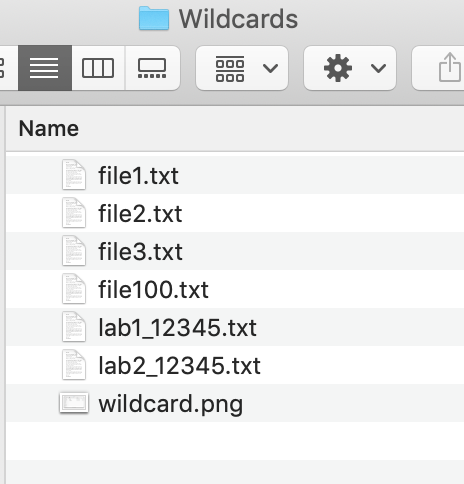
\includegraphics[width=0.3\textwidth]{img/files.png}
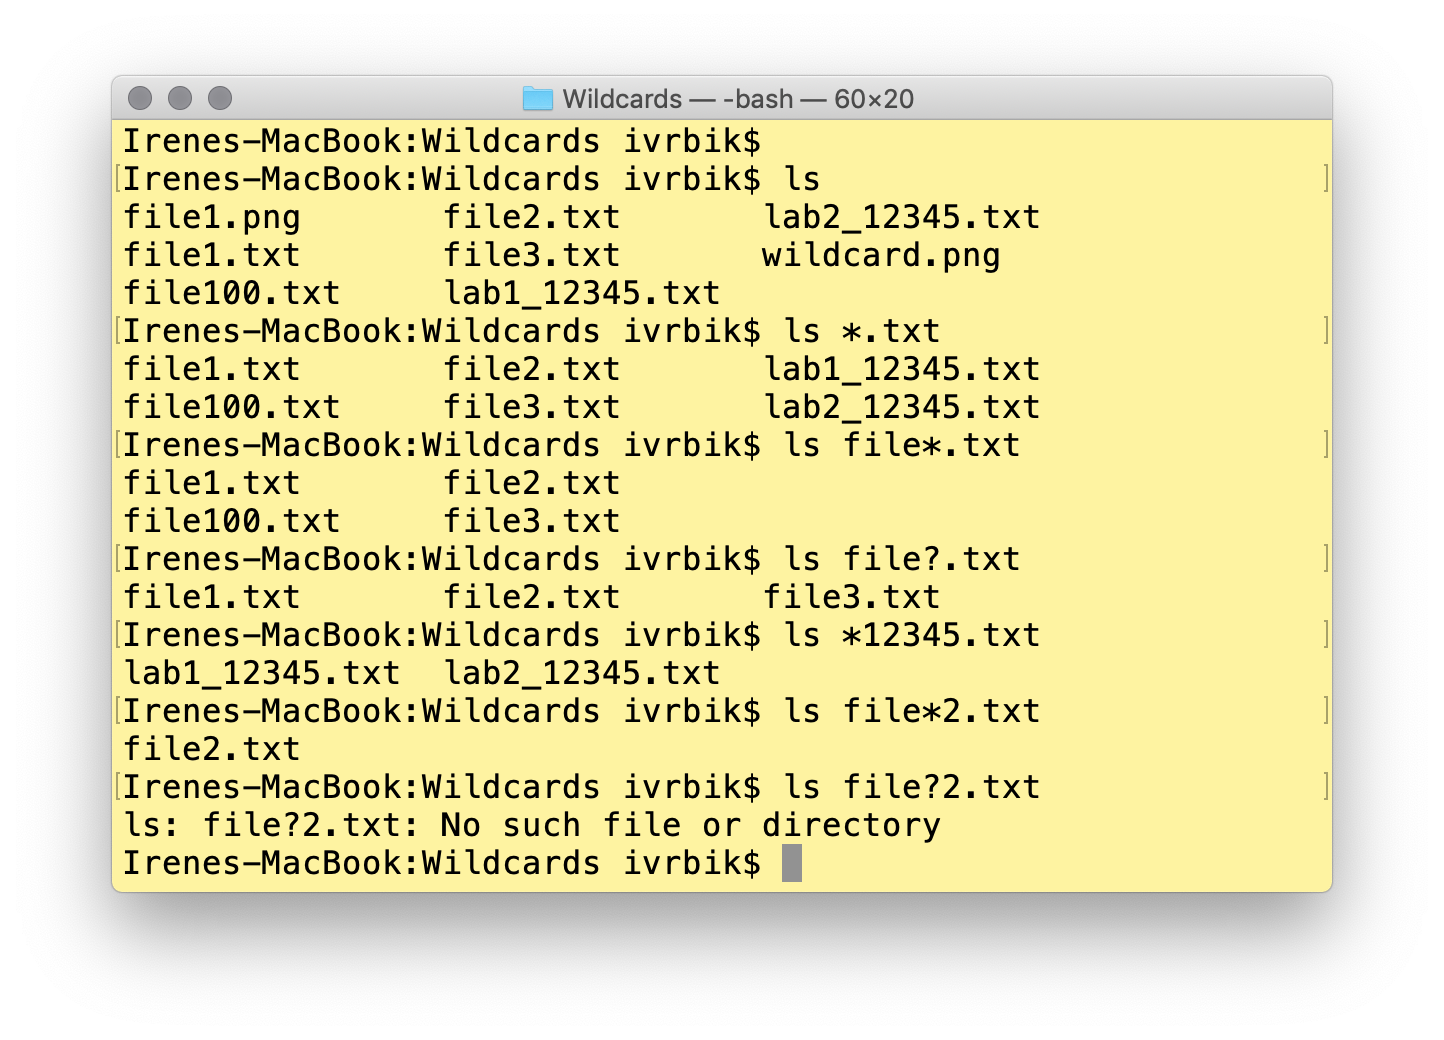
\includegraphics[width=0.7\textwidth]{img/wildcards.png}

Replace {\tt ls} with {\tt dir} if you are using Windows.
\end{frame}



\begin{frame}\ft{Navigating the Command Line}
\begin{tabular}{|l|l |l |}
\hline
&\multicolumn{1}{c|}{\bf Windows} & \multicolumn{1}{c|}{\bf Mac OS \& Linux}\\
\hline 
Previous command in history
& Up
& Up\\
Next command in history
& Down
& Down\\
First command in history
& PageUp
& \\
Last command in history
& PageDown
& \\
Move to start of line
& Home
& Ctrl+A\\
Move to end of line
& End
& Ctrl+E\\
Auto-compete file name
& Tab
& Tab\\
\hline
\end{tabular}
%Other windows:
%-  Esc - Clears the current command 
%F7 - Displays the command history in a scrollable pop-up box 
%F8 - Displays commands that start with characters currently on the command line 
%Alt+F7 - Clears the command history 


%{background:#ddd}. |_. Key/Command |_. Description |
%| Tab | Auto-complete files and folder names |
%| Ctrl + A | Go to the beginning of the line you are currently typing on |
%| Ctrl + E | Go to the end of the line you are currently typing on |
%| Ctrl + U | Clear the line before the cursor |
%| Ctrl + K | Clear the line after the cursor |
%| Ctrl + W | Delete the word before the cursor |
%| Ctrl + T | Swap the last two characters before the cursor |
%| Esc + T | Swap the last two words before the cursor |
%| Ctrl + R | Lets you search through previously used commands |
%| Ctrl + L or Command + K | Clears the Screen |
%| Ctrl + C | Kill whatever you are running |
%| Ctrl + D | Exit the current shell |

\end{frame}

\begin{frame}\ft{Pausing or Cancelling Commands}
To \define{pause} a command:
\begin{description}
\item[Windows:] Press \keystroke{Ctrl}+\keystroke{S} or the \keystroke{Pause} To resume, press any key. 
\item[Mac:] \keystroke{Ctrl}+\keystroke{Esc} or \keystroke{Cmnd}+\keystroke{.}\nl
\end{description}


To \define{cancel} a command, press \keystroke{Ctrl}+\keystroke{C}.% or \keystroke{Ctrl}+\keystroke{Break}.
\begin{itemize}
\item The command is canceled, and the command prompt returns.
\item However, any actions performed before the cancel are not undone.
\end{itemize}
\end{frame}



%%%%%%%%%%%%%%%%%%%%%%%%%

% question:

\begin{frame}\ft{}
  \begin{example}
How many of the following statements are TRUE?
\begin{enumerate}
\item {{To cancel a command, press \keystroke{Ctrl}+\keystroke{X}.
}}
\item {{To go to the most recent command, press Up arrow.
}}
\item {{This wildcard expression {\tt te*a?.txt} matches {\tt tea12.txt}.
}}
\item {{The command to change a directory is {\tt pwd}.
}} 
\end{enumerate}
\begin{multicols}{5}
\begin{enumerate}[A)]
\item 0 
\item 1
\item 2
\item 3
\item 4
\end{enumerate}
\end{multicols}
  \end{example} 
\end{frame}


% answer:

\begin{frame}<handout:0>\ft{}
  \begin{block}{Answer:}
How many of the following statements are TRUE?
\begin{enumerate}
\item {\color<2->{red}	{To cancel a command, \keystroke{Ctrl}+\keystroke{X}.}}
\item {\color<3->{sgreen}	{To go to the most recent command, press Up arrow.
}}
\item {\color<4->{red}	{This wildcard expression {\tt te*a?.txt} matches {\tt tea12.txt}.
}}
\item {\color<5->{red}	{The command to change a directory is {\tt pwd}.
}} 
\end{enumerate}
\begin{multicols}{5}
\begin{enumerate}[A)]
\item 0
\item \tans{5}{1} 
\item 2
\item 3
\item 4
\end{enumerate}
\end{multicols}
  \end{block} 
\end{frame}


%%%%%%%%%%%%%%%%%%%%%%%%%






\begin{frame}\ft{Try It: Navigating Directories with Commands}
\begin{example}{}
Using a terminal window, perform the following actions:
\begin{enumerate}
\item Create a directory called 301.
\item Change into the directory 301.
\item Echo I am awesome!
\item Show your current directory (print working directory).
\item Create a text file called message.txt with a message in it.
\item List the contents of your directory.
\item Rename the file message.txt to test.txt.  Verify the name change.
\item Delete the test.txt file.
\item Change directory to directory above 301.
\item Delete directory 301.
\end{enumerate}
\end{example}
\end{frame}

\begin{frame}\ft{Command Arguments - Windows}
A command can take \emph{arguments} that changes its behaviour.
\begin{itemize}
\item Example: \orange{Path} was an argument for the cd command. 
 {\tt cd \orange{301}}\nl
\end{itemize}

On Windows, commands also can be modified by a \emph{switch} (or extension) which is usually a slash then a letter (e.g. {\tt /S}).
\begin{itemize}
\item To find out what is available, run the command with: {\tt /?}
\end{itemize}
$$\ipic{help}{0.99}$$
\end{frame}

\begin{frame}\ft{Command Arguments - Mac/Linux}
On Mac/Linux arguments are separated by spaces and begin with `{\tt -}' \nl
An explanation of arguments can be found by using man then the command name.  Example: {\tt man cp} (to \textit{quit} press {\tt q})
\begin{center}
\ipic{man}{0.7}
\end{center}
\end{frame}

\begin{frame}\ft{Standard Input, Output, and Error}
\define{Standard input} ({\tt stdin}) is the default input device (usually a keyboard) into the terminal.\nl

\define{Standard output} ({\tt stdout}) is the location where output is sent after a command is run.  The default is the terminal window.\nl

\define{Standard error} ({\tt stderr}) is the location where error messages are displayed (typically the terminal window).

\end{frame}

\begin{frame}\ft{Redirecting Input}
By default, a command gets its input from standard input and outputs results to standard output.\nl

A command can get its input from the output of another command by using the \define{pipe} (\define{|}) symbol.  Example:
\begin{center}
{\tt cat test.txt | \purple{wc}}
\end{center}
Note the example commands are Mac OS/Linux only: {\tt \purple{wc}} (word count) is not on Windows.\nl

Also can use redirect input (<) to send input to a command.  Ex:
\begin{center}
{\tt cat < test.txt}
\end{center}
same as
\begin{center}sort
{\tt cat test.txt}
\end{center}
%Note that we can chain together multiple pipes.


\end{frame}

\begin{frame}\ft{Redirecting Output}
Redirect output using {\tt >} which will overwrite the file:
\begin{center}
 {\tt sort test.txt > sorted.txt}
\end{center}



Use{\tt >>} to append to the existing file:
\begin{center}
{sort test.txt >> sorted.txt}
\end{center}


\end{frame}


\begin{frame}{Redirection Summary}
\begin{center}
\begin{tabular}{|l|c|}
\hline
& {\bf Symbol}\\\hline
Redirect input & 
{\tt <} \\
Redirect output
& {\tt >} \\
Redirect output (append)
& {\tt >}{\tt >}\\
Pipe output to input of next command
& {\tt |}\\\hline
\end{tabular}
\end{center}
\end{frame}

\begin{frame}[fragile]\ft{Escape Symbol}
An \emph{escape symbol} is used when a command requires input that contains a character with a special meaning.  The escape symbol indicates this character is data not part of the command.
\begin{description}
\item[Windows] the caret (\verb!^!) indicates that whatever character that follows it is data rather than part of the command. 
\begin{itemize}
\item Example:  \verb!cp test.txt a^&b.txt!
\end{itemize}
\item[Linux] use the backslash (\verb!\!).\nl
\end{description}

This is especially common when dealing with spaces in a file name.  The other way to handle file names with spaces is to enclose them in double \href{http://wiki.bash-hackers.org/syntax/quoting
}{quotes}:
$$\verb!cp test.txt "c:\program files\file spaces.txt"!$$
\end{frame}

\begin{frame}\ft{Environment Variable}
\define{Environment variables} allow for customization and control of the command and system environment.\nl

Current variables are seen using the {\tt set} or {\tt env} command.\nl

Important variables:
\begin{description}
\item[{\tt\$PATH}] list of directories where commands/applications will be found
\item[{\tt \$HOME}]  user home directory
\end{description}
\end{frame}

\begin{frame}\ft{Finding Text in Files}
The {\tt grep} command allows for searching for text in files that match a pattern (Mac/Linux only, {\tt find} on Windows).
\begin{itemize}
\item {\tt grep} stands for "global regular expression print"
\item Search is case-sensitive (use {\tt -i} for case-insensitive) and can contain regular expressions.
\begin{itemize}
\item {\tt grep -i} will be case-insensitive
%\item {\tt grep -R} will search all files in directory\nl
\end{itemize}
\end{itemize}

Example:
\begin{center}
{\tt  grep er *.txt}
\end{center}
searches for {\tt er} in any file that ends in {\tt .txt}
%Windows: find "er" *.txt
\end{frame}

\begin{frame}\ft{Batch Files}
A \define{batch program} (also commonly called a \emph{batch file} or \emph{command file}) is a text file that contains a sequence of commands to be executed.\nl

You define the sequence of commands, name the sequence, and then execute the commands by entering the name at a command prompt.  Any action you can take by typing a command at a command prompt can be encapsulated in a batch program. \nl

In Windows files typically end in {\tt.bat} or {\tt.cmd} and on Mac/Linux with {\tt.sh}\nl
Batch files can take arguments like other commands.

\end{frame}

\begin{frame}\ft{Connecting to Another Computer using SSH}
\define{Secure shell} or \emph{SSH} is a protocol allowing remote login to other machines to execute commands.
\begin{itemize}
\item The network communication is encrypted for security.
\item An open-source program on campus is Putty.\nl
\end{itemize}

Using SSH allows you to connect and execute commands on another machine even when you do not have physical access to that machine.\nl

SSH may be used to send or retrieve data from other computers for analysis.

\end{frame}

\begin{frame}[fragile]\ft{Try it: Using Batch Files}
Before creating the batch file, create a file called {\bf numbers.txt} that has the numbers {\tt one, two, three, ... , ten}.
\begin{example}
Using a terminal window, create a batch file called {\bf myscript.bat} (or {\bf .sh}), to perform the following:
\begin{enumerate}
\item  sort {\bf numbers.txt} and output as {\bf sorted.txt}.
\item output the word count on {\bf numbers.txt} to {\bf count.txt}.
\item take {\bf numbers.txt} and append its data three times into the file {\bf output.txt}.
\item search for \verb|"e"| in {\bf output.txt} and write results as file {\bf search.txt} (use {\tt grep}).
\item Output the contents of {\bf sorted.txt}, {\bf output.txt}, and {\bf search.txt} .
\item Run your batch file.
\end{enumerate}
\end{example}

\end{frame}

\begin{frame}\ft{Conclusion}
The \emph{command line} is the text interface to the computer that accepts commands that the computer will execute including running programs, manipulating files, and running scripts.\nl

The command line allows for automation and more control than may be available in the user interface.  It may also be the only way to interact with the machine if connecting via SSH.\nl

The command environment allows for redirecting the standard input and output using input/output redirection and pipes.

\end{frame}

\begin{frame}\ft{Objectives}
\begin{itemize}
\item Define command line and list some of its uses
\item Explain the purpose of an operating system
\item Know how to open the command line window on Mac OS and Windows
\item Be able to enter commands and stop them
\item Define: file system, folder, file
\item Explain the difference between an absolute and relative path
\item Use command line shortcuts to save time
\item Be able to match wildcards involving ? and *
\item Be able to cancel a command
\end{itemize}

\end{frame}

\begin{frame}\ft{Objectives cont'd}
\begin{itemize}
\item Explain standard input, standard output, and standard error
\item Be able to use input and output redirection and pipes (?, >, < , >>)
\item Explain the reason for an escape symbol
\item Define and explain the purpose of environment variables.
\item Be able to use grep to search text files.
\item Explain the purpose of a batch program.
\item Be able to connect to another machine using SSH. 
\end{itemize}
\end{frame}


\begin{frame}
  {Questions}

  \nocite{lorem,ipsum}
  \bibliographystyle{plain}
  \bibliography{../demo}

\end{frame}

\end{document}

